% THIS IS SIGPROC-SP.TEX - VERSION 3.1
% WORKS WITH V3.2SP OF ACM_PROC_ARTICLE-SP.CLS
% APRIL 2009
%
% It is an example file showing how to use the 'acm_proc_article-sp.cls' V3.2SP
% LaTeX2e document class file for Conference Proceedings submissions.
% ----------------------------------------------------------------------------------------------------------------
% This .tex file (and associated .cls V3.2SP) *DOES NOT* produce:
%       1) The Permission Statement
%       2) The Conference (location) Info information
%       3) The Copyright Line with ACM data
%       4) Page numbering
% ---------------------------------------------------------------------------------------------------------------
% It is an example which *does* use the .bib file (from which the .bbl file
% is produced).
% REMEMBER HOWEVER: After having produced the .bbl file,
% and prior to final submission,
% you need to 'insert'  your .bbl file into your source .tex file so as to provide
% ONE 'self-contained' source file.
%
% Questions regarding SIGS should be sent to
% Adrienne Griscti ---> griscti@acm.org
%
% Questions/suggestions regarding the guidelines, .tex and .cls files, etc. to
% Gerald Murray ---> murray@hq.acm.org
%
% For tracking purposes - this is V3.1SP - APRIL 2009

\documentclass{acm_proc_article-sp}

\usepackage{listings}
\lstset{breaklines=true}
\lstset{numbers=left, numberstyle=\scriptsize\ttfamily, numbersep=10pt, captionpos=b} 
\lstset{basicstyle=\small\ttfamily}
\lstset{framesep=4pt}

\begin{document}

\title{Evolving Fighting Creatures: A Look into Fitness and Competitive Coevolution\titlenote{The full project lives at https://github.com/coch9894/Evolving-Fighting-Creatures}}
%
% You need the command \numberofauthors to handle the 'placement
% and alignment' of the authors beneath the title.
%
% For aesthetic reasons, we recommend 'three authors at a time'
% i.e. three 'name/affiliation blocks' be placed beneath the title.
%
% NOTE: You are NOT restricted in how many 'rows' of
% "name/affiliations" may appear. We just ask that you restrict
% the number of 'columns' to three.
%
% Because of the available 'opening page real-estate'
% we ask you to refrain from putting more than six authors
% (two rows with three columns) beneath the article title.
% More than six makes the first-page appear very cluttered indeed.
%
% Use the \alignauthor commands to handle the names
% and affiliations for an 'aesthetic maximum' of six authors.
% Add names, affiliations, addresses for
% the seventh etc. author(s) as the argument for the
% \additionalauthors command.
% These 'additional authors' will be output/set for you
% without further effort on your part as the last section in
% the body of your article BEFORE References or any Appendices.

\numberofauthors{2} %  in this sample file, there are a *total*
% of EIGHT authors. SIX appear on the 'first-page' (for formatting
% reasons) and the remaining two appear in the \additionalauthors section.
%
\author{
% You can go ahead and credit any number of authors here,
% e.g. one 'row of three' or two rows (consisting of one row of three
% and a second row of one, two or three).
%
% The command \alignauthor (no curly braces needed) should
% precede each author name, affiliation/snail-mail address and
% e-mail address. Additionally, tag each line of
% affiliation/address with \affaddr, and tag the
% e-mail address with \email.
%
% 1st. author
\alignauthor
Alex Cochrane\\
       \affaddr{University of Idaho}\\
       \email{coch9894@vandals.uidaho.edu}
% 2nd. author
\alignauthor
Jordan Leithart\\
       \affaddr{University of Idaho}\\
       \email{leit7193@vandals.uidaho.edu}
}
% There's nothing stopping you putting the seventh, eighth, etc.
% author on the opening page (as the 'third row') but we ask,
% for aesthetic reasons that you place these 'additional authors'
% in the \additional authors block, viz.

% Just remember to make sure that the TOTAL number of authors
% is the number that will appear on the first page PLUS the
% number that will appear in the \additionalauthors section.

\maketitle
\begin{abstract}

An essential part of any genetic program is the use of a well defined fitness function that produces the desired outputs. For competitive coevolution this does not change. However, the ability to view the affects of different fitness functions on two simultaneously evolving populations can be seen through competition. Through competition, the value of a good fitness function will become apparent from the winner of the competition. We propose that it is possible to see the affects of different fitness functions through control of an individuals fitness which then can be normalized to compare to other individuals fitnesses in the population. We would like to see if logical fitness functions are always the best at producing good results and if training and testing have any affect on the appearance of the Red Queen Effect.

Through experimentation using a genetic program, we were able to observe that logical fitness functions do perform better, but not to the degrees that we would have expected. Similarly, only similar strategies seemed to be affected by the Red Queen Effect namely, attempting to maximize hits on the opponent. Fitness functions were also very reliant on their opponent, which caused random behavior to exhibit through the ability of poor fitness functions to occasionally be successful and win against a logical fitness function.

\end{abstract}

% A category with the (minimum) three required fields
%\category{H.4}{Information Systems Applications}{Miscellaneous}
%A category including the fourth, optional field follows...
%\category{D.2.8}{Software Engineering}{Metrics}[complexity measures, performance measures]

%\terms{}

\keywords{Genetic Programming, Coevolution, Competitive Coevolution, Evolutionary Computation, Red Queen Effect, Fitness Function} % NOT required for Proceedings

\section{Introduction} % Include Papers here

Fitness is the driving force of evolutionary computation. Unfortunately, they are also the most computationally expensive process within evolutionary computation. To solve this problem approximate models were created that were computationally efficient\cite{Fitness}. What we want to look at for our experiment is the effectiveness of fitness functions and their ability to perform against each other. Relating this to approximate models of fitness, which are usually assumed to be correct\cite{Fitness}, we can see that the method for an approximate model will only be correct when the approximate model itself is globally correct. For our experiment we want to see if their is a correlation between logically correct strategies and winning competitions. Our fitness functions will differ in the way they value different aspects of an individual. To compare them however we had a need to create a normalizing function. More on these methods will be covered later. 

A big part of our project deals with the Red Queen Effect. The Red Queen Effect deals with the idea that a population may be improving some trait, even though their fitness might remain constant\cite{Ebner}. Previous work done by Marc Ebner\cite{Ebner} states that before his work on evolving artificial plants in a single population, the usual setting for the Red Queen Effect was a predator population versus a prey population\cite{Ebner}\cite{Red}. Ebner states that ecological interactions are an important part evolution. In Ebner's plant ecosystem, it was common to see a fluctuating fitness around a constant level that sometimes even decreased.

For our experiment, we would like to drop the distinction of predator and prey from the individuals. Instead we would like to look at the strategies of an individual and whether those strategies are effected by the Red Queen Effect. Our creatures who are fighting will only be distinguished by their strategy. This strategy will be developed by the differences in their fitness function. Therefore during evaluation we will compare two individuals at a time. Our engine will allow us to compare any two individuals we want with no bias going to either side.

What we would like to see is the Red Queen Effect disappear from our project because of our method of training and testing. Our project will go through a set number of rounds. A normal round will have a single population evaluating against other members of that same population. Every 10 rounds however we will evaluate a population against another. This will hopefully change the strategy of both populations and help them improve their fitnesses by keeping their opponents inconsistent. This method is similar to that of \textit{evolution control}\cite{Fitness}.

Evolution control deals with evaluating with both an original fitness function and an approximate function. One of its methods is to have control individuals who use the original fitness function. While evaluating, the approximate function is used except for at a set interval where the control or original function is used to produce control individuals. In our case our original fitness functions is to compare fitness functions and have individuals from two differing populations compete.

One thing that we want to do is be able to know what the best is at any given time. This has been looked at before and is called a master tournament\cite{Red}. The master tournament takes the best individuals and saves them at each generation so they can be tested against at the very end. For us we would like to use this idea for a similar purpose. We would like to see optimization happen. That is what our different fitness functions are really for.

While Ebner saw a fluctuating fitness around a constant value in his results\cite{Ebner}, we hypothesize that by keeping opponents inconsistent and varying we can see a small yet steady improvement in one populations best fitness. This best fitness is representative of an individual that has been trained to handle similar strategies to his own, but can still beat differing strategies. A final test will to test this individual against a saved set of best individuals from each round. If the best individual can pass a large majority of the tests (greater than 90\%), our hypothesis will be justified. If it cannot pass our hypothesis will have failed.

\section{The Experiment} % BODY

The simplest way to test our hypothesis was to build a genetic program that could be used in conjuncture with a graphics engine so our end results could be shown and quantified. To do so we built a genetic program that would evolve the instructions for an individual. To evaluate these individuals with different fitness functions it seemed best to use the idea of training two populations on separate fitness functions and then testing them against each other at regular intervals to get a grasp on the validity of each fitness function. After each generation, the best individual from \textit{either} population was saved into a separate population as a control group. When evolution ended, the best individual was tested against this control group to check for the Red Queen Effect. This allowed us to observe if we were creating a overall best solution or if we were cycling through a few strategies.

\subsection{Individuals} % What makes an individual
Our individuals were made up of common and new behaviors that we needed to model our creatures. The following list of Non-Terminals and Terminals is all we used to make up our individual. Evolution was the key to setting them in the correct order and will be covered in the next section.
\begin{itemize}
\item Non-Terminals
	\begin{itemize}
	\item Prog2 - When called during evaluation, pushes its left child, then its right child onto the correct player stack.
	\item Prog3 - When called during evaluation, pushes its left child, middle child, then its right child onto the correct player stack.
	\end{itemize}
\item Terminals
	\begin{itemize}
	\item Move - When called during evaluation, moves the correct players x position by cos(this->direction)* speed + 0.5 where the direction is where the player is facing. Also moves the correct players y position by sin(this->direction)*speed + 0.5.
	\item Turn Left - When called during evaluation, computes this->direction += BASE\_ANGLE which changes the direction the player is facing.
	\item Turn Right - When called during evaluation, computes this->direction -= BASE\_ANGLE which changes the direction the player is facing.
	\item Aim - When called during evaluation, computes the angle to turn by using the current position of both players and the arc-tangent. In other words, we set the angle to turn to be atan( (y2-y1)/(x2-x1) ).
	\item Shoot - When called during evaluation, adds a new bullet to the environment list containing environment variables.
	\end{itemize}
\end{itemize}

\begin{table*}
\centering
\caption{Evolutionary Characteristics}
\label{evochar}
\begin{tabular}{|l|p{4in}|}
\hline
Algorithm & Generational\\
\hline
Population size & 15 Players\\
\hline
Selection method & Tournament Select (tournament size was 2)\\
\hline
Elitism & Yes, the best individual per generation was copied over\\
\hline
Crossover method & Subtree crossover\\
\hline
Crossover rate & We took a random integer whose range was the size of each parent, then traversed the tree in a depth-first method. When I had visited the number of nodes equal to that random integer We crossed over on that node.\\
\hline
Mutation method & Node mutation; 10\% chance that each node in each individual would be mutated\\
\hline
Operator/non-terminal set & \{prog3, prog2\}\\
\hline
Terminal set & \{rotate left, rotate right, aim, move forward, shoot\}\\
\hline
Fitness function 1 & MaxMax; The goal of this training fitness was to maximize the number of times the opponent was hit by the player's bullets, and to maximize the number of times the player was hit. \\
\hline
Fitness function 2 & MinMax; The goal of this training fitness was to minimize the number of times the opponent was hit by the player's bullets, and to maximize the number of times the player was hit. \\
\hline
Fitness function 3 & MinMin; The goal of this training fitness was to minimize the number of times the opponent was hit by the player's bullets, and to minimize the number of times the player was hit. \\
\hline
Fitness function 4 & MaxMin; The goal of this training fitness was to maximize the number of times the opponent was hit by the player's bullets, and to minimize the number of times the player was hit. \\
\hline
\end{tabular}
\end{table*}

\subsection{Elitism}
To maintain the best players across generations, we decided to create an elite for each generation. This elite was pitted against every other player in the population to ensure that it was indeed the best player. Each elite was chosen based on the training fitness assigned to that specific search, see Table \ref{evochar}. This particular area of our program was where most of the time was spent. We had to check each player against every other player which added up computational power quickly. Once we had gathered all the fitness, we averaged it out and returned the better player The following is pseudo code for our get elite function:
\begin{lstlisting}
  Player *one;
  Player *two;
  for(int i = 0; i < POP_SIZE - 1; i++){
    one = pop->GetIndividual(i);
    for(int j = i+1; j < POP_SIZE; j++){
      two = pop->GetIndividual(j);
      Evaluate(one, two, false);
      pop->fitnessPopulation[i] += one->GetTrainingFitness();
      pop->fitnessPopulation[j] += two->GetTrainingFitness();
    }
    pop->fitnessPopulation[i] = pop->fitnessPopulation[i]/POP_SIZE;
  }
  pop->fitnessPopulation[POP_SIZE] = pop->fitnessPopulation[POP_SIZE]/POP_SIZE;
  int winningIndex = 0;
  for(int i = 0; i < POP_SIZE; i++){
    if(pop->fitnessPopulation[winningIndex] < pop->fitnessPopulation[i]){
      winningIndex = i;
    }
  }
  return pop->GetIndividual(winningIndex);
\end{lstlisting}

\subsection{Tournament Select}
The tournament select function grabbed two random players. Then, it evaluated the two players against each other. We specifically made it so that the players could not be the same player. The tournament select then compared their fitness (based on the training fitness used for that specific genetic program), and selected whichever one was better. The following is pseudo code for our tournament select function:
\begin{lstlisting}
  int oneIndex = rand()%POP_SIZE;
  int twoIndex = rand()%POP_SIZE;

  while(oneIndex == twoIndex){
    oneIndex = rand()%POP_SIZE;
  }

  Player *one = pop->GetIndividual(oneIndex);
  Player *two = pop->GetIndividual(twoIndex);
  Evaluate(one, two, false);
  if(two->GetTrainingFitness() > one->GetTrainingFitness()){
    return twoIndex;
  }

  return oneIndex;
\end{lstlisting}

\subsection{Crossover}
The crossover function took the two winners of the above tournament select and crossed over at a random number, see Table \ref{evochar}. This algorithm performed a depth-first traversal through the player tree. Once it arrived at the random node, it crossed over with the second player. The actual crossover algorithm required a deep copy of the subtree to be made and then attached. We used a temporary tree to hold that subtree and then attached it by setting the parent node equal to the tmpParent's node. Here is some pseudo code to explain this:
\begin{lstlisting}
  node *tmpNode = firstNode->copyTree(firstNode, firstNode->parent);
  firstNode = firstNode->copyTree(secondNode, firstNode->parent);
  secondNode = secondNode->copyTree(tmpNode, secondNode->parent);
\end{lstlisting}

\subsection{Mutation}
The mutation function traversed the player tree in a depth-first traversal. At every node, a random number between 1 and 100 was generated. If the number was less than 10, the current node was mutated. To make sure that the node didn't change types (terminal to non-terminal and visa versa), if the node was a terminal a random terminal node was generated. Because we only had two non-terminals in our set, see Table \ref{evochar}, we just switched prog3 over to prog2 and visa versa.

\subsection{Evaluate}
The evaluate function was the meat of our genetic program. It took in two separate players and pitted them against each other, counting up the number of times each player was hit. Because our player tree (which had all of our actions in it), was in a separate class from the player class, we had to create a depth-first traversal without using recursion. To do this effectively, we had to use a stack data structure. By pushing right to left, and then popping the top off we were able to simulate a recursive depth-first traversal. In the interest of time, we gave each player only 300 actions. This number would be decreased every time an action was performed to ensure that only 300 actions were taken.

\subsection{Fitness \& Other Algorithms} % Fitness etc.

To keep the fitnesses simple we decided to keep track the number of times an individual hit the opponent and the number of times that an opponent hit the individual. These were the numbers that our fitness functions would try to control. For example we might want to try and maximize the number of successful hits of the opponent and maximize the number of times the opponent hits the individual. In theory this doesn't sound like that great of a strategy but maybe against some other fitness function it would be great.

When we would like to compare the different functions however we needed some way to standardize these fitnesses. We came up with what we viewed as a perfect fitness and created a normalizing function to use the two prior values to represent it. Therefore our fitness functions are really controlling methods and strategies for getting the highest normalized fitness. The following is pseudo code for our normalization function:
\begin{lstlisting}
    if(this->numSuccess == this->numFail)
    {
        this->fitness = 1;
    }
    else
    {
        if(this->numFail == 0){
            this->numFail += 0.01;
        }
        this->fitness = numSuccess/numFail;
    }
\end{lstlisting}
Because we decided to use a division of Success/Failures, we had to account for 0 in the denominator. Therefore if the Successes=Failures we just set our "stalemate" value or "average" outcome at 1. Therefore anything over 1 is assumed to be above average during the division. If the denominator is 0 and the numerator is not, we take this as an exceptionally good individual and wish to divide by 0.01 which essentially multiplies our answer by 100.

\subsubsection{Fitness Functions}

As seen in Table \ref{evochar}, we will be testing our hypothesis using four different fitness functions. Since the fitness functions are how we will control our strategies we wanted to keep them basic in their functionality. Therefore, we settled on maximizing and minimizing the success and failures. By doing this, we can see if a logical solution like maximizing an individuals hits on an opponent and minimizing an opponents hit on itself, is as good in simulation as we logically would think it would be.

\subsubsection{Turning Logic} % Our Turn_Left and Turn_Right Logic

When training or testing to obtain fitness, it is unknown which side of the board the individual will be on or if they will always be on the same side of the board. To compensate for this, when a player is designated to be Player1, a turn\_left action will cause them to rotate their facing direction in a positive direction and a turn\_right action will cause them to rotate their facing direction in a negative direction. However, when a player is designated as Player2, a turn\_left action will cause them to rotate their facing direction in a negative direction and a turn\_right action will cause them to rotate their facing direction in a positive direction. This removes any chance of an individual evolving a strategy for only one side of the board. This will help create a universal strategy.

\section{Results} % Results

Due to time constraints, we observed only MaxMax vs the rest of the fitness functions, see Table \ref {evochar}, this was an excellent choice because we expected that MaxMax would be second best. We observed that it was in actuality the best fitness function. We discovered this was due to MaxMax always being on the left hand side of the board, and in our evaluation function the left side won all ties. This was especially prevalent in the results between MaxMax vs. MaxMin, see subsection \ref{MAXMAXvMAXMIN}.

\subsection{MAXMAX VS. MINMAX}
\label{MAXMAXvMINMAX}
We expected that MaxMax would dominate this matchup, winning every single competition. However, this was not observed fully. We did see a dominant player in MaxMax, see Figure \ref{fig:MaxMaxMinMax}, which won 90\% of the matchups. We believe that the MinMax player evolved a strategy halfway through that moved and shot and the MaxMax player evolved a stand and shoot strategy.
\begin{figure}[h]
\centering
\caption{MaxMax vs. MinMax}
\label{fig:MaxMaxMinMax}
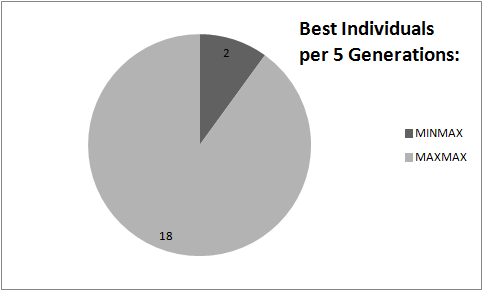
\includegraphics[width=0.5\textwidth]{MaxMaxvMinMax}
\end{figure}

\subsection{MAXMAX VS. MINMIN}
\label{MAXMAXvMINMIN}
Similar to subsection \ref{MAXMAXvMINMAX} we expected that MaxMax would dominate this matchup as well. We also expected it to win every single competition. Again, this was not observed fully, with MaxMax actually performing worse and MinMin winning 20\% of the matchups. This was a shocking revelation because we didn't expect MinMin to evolve a shooting function at all, so we must assume that in those particular generations every individual in MinMin had evolved a shooting function, and in the same generation MaxMax had devolved from a stand and shoot behavior that we were expecting. However, once we had evolved to our maximum generations, we noticed that MaxMax had re-evolved a stand and shoot fighting strategy, see Figure \ref{fig:pic2}.
\begin{figure}[h]
\centering
\caption{MaxMax vs. MinMin}
\label{fig:MaxMaxMinMin}
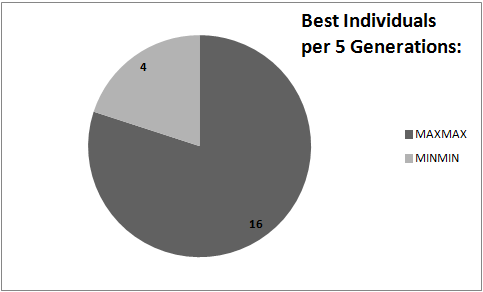
\includegraphics[width=0.5\textwidth]{MaxMaxvMinMin}
\end{figure}

\subsection{MAXMAX VS. MAXMIN}
\label{MAXMAXvMAXMIN}
Based off the fitness functions in Table \ref{evochar}, and since the normalized fitness function was the fitness function that MaxMin was training on, we expected that MaxMin would win this matchup, but not necessarily dominate. In this matchup, we expected to see more of a Red Queen Effect due to similarities in trying to maximize hits on the opponent. What we observed was that the two players tied a few times, with the tie going to MaxMax due to it being on the left, otherwise they were evenly matched with MaxMax holding a slight edge, assumed due to the ties. We also observed periods of behavior where one player would win several generations in a row before the other player solved that strategy.
\begin{figure}[h]
\centering
\caption{MaxMax vs. MaxMin}
\label{fig:MaxMaxMaxMin}
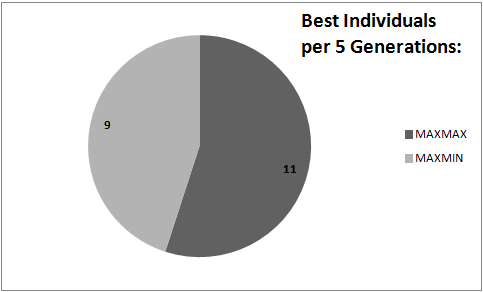
\includegraphics[width=0.5\textwidth]{MaxMaxvMaxMin}
\end{figure}

\section{Conclusions} % Conclusions

First off, our hypothesis that we would be able to see a small, steady improvement in a populations best individual was not true. We observed that some seemingly random behaviors no matter what generation we were on. We believe that this is due to having no conditionals in our non-terminal set. Without these conditionals code bloat did not occur so every sub-tree was acted upon. If we were to perform this experiment again we would add a conditional to the non-terminal set such as, if\_recently\_shot or if\_opponent\_hit. We believe this would allow for inoperable code to be hidden and therefore crossover and mutation would not have such drastic affects each generation.

Secondly, while we did not have a master tournament\cite{Red} at the end of our competitions, we attempted a red robin tournament that had similar effects. During this tournament we observed the Red Queen Effect as seen in Table 2. %\ref{tMAXMAXvMAXMIN}
In the table you can clearly see winner rotation with nearly a 50\% split. This also means that our hypothesis that the red queen effect would not be present if training and testing were done separately is wrong. However, we were able to show that fitness function MaxMax had no Red Queen Effect when evaluated against any fitness function except MaxMin. Therefore we conclude that only similar strategies are effected by the Red Queen Effect in this type of tournament.

Lastly, we ran into a problem were our program slowed down significantly as we continued to search across the landscape. We observed that in the 4th search, MinMin vs MinMax, it took 12 hours to finish 30 generations. If we had more time, we would combat this by gathering the data for each search individually, instead of all at once. This setback caused us to have to extrapolate data across our round robin style tournament. We feel we can safely assume that MaxMin would perform similarly to MaxMax when evaluating against all the other fitness functions, because of ties and how only similar strategies seem to be affected by the Red Queen Effect.

\begin{table}[h]
\centering
\label{tMAXMAXvMAXMIN}
\caption{MaxMax vs. MaxMin}
\begin{tabular}{|l|p{1in}|}
\hline
\textbf{MaxMin} & 11.5 \\
\hline
\textit{MaxMax} & 0 \\
\hline
\textit{MaxMax} & 1 \\
\hline
\textit{MaxMax} & 900 \\
\hline
\textit{MaxMax} & 3200 \\
\hline
\textbf{MaxMin} & 1.92391 \\
\hline
\textit{MaxMax} & 1 \\
\hline
\textit{MaxMax} & 2600 \\
\hline
\textbf{MaxMin} & 1 \\
\hline
\textit{MaxMax} & 0.333333 \\
\hline
\textbf{MaxMin} & 0.974684 \\
\hline
\textbf{MaxMin} & 2600 \\
\hline
\textbf{MaxMin} & 3.5 \\
\hline
\textbf{MaxMin} & 1.22222 \\
\hline
\textbf{MaxMin} & 0.495575 \\
\hline
\textit{MaxMax} & 2.0625 \\
\hline
\textit{MaxMax} & 2100 \\
\hline
\textbf{MaxMin} & 1.35294 \\
\hline
\textit{MaxMax} & 1.11111\\
\hline
\textit{MaxMax} & 1.1 \\
\hline
\end{tabular}
\end{table}

%
% The following two commands are all you need in the
% initial runs of your .tex file to
% produce the bibliography for the citations in your paper.
\bibliographystyle{abbrv}
\bibliography{sigproc}  % sigproc.bib is the name of the Bibliography in this case
% You must have a proper ".bib" file
%  and remember to run:
% latex bibtex latex latex
% to resolve all references
%
% ACM needs 'a single self-contained file'!
%
%APPENDICES are optional
%\balancecolumns

%ACKNOWLEDGMENTS are optional
\section{Acknowledgements}
We would like to especially thank Dr. Terrence Soule for his help and guidance during this project. His help in finding resources was invaluable. We would also like to thank Jordan's CPU for never dying during its 72 hour marathon to gather our relevant data.

\appendix
%Appendix A
\section{Graphics}

\paragraph{} Here are a few screenshots of the first two searches in action. Figure \ref{fig:pic} shows the MaxMax in action versus the MinMax. Refer to Table \ref{evochar} to see what type of functions are being used. Figure \ref{fig:pic2} shows a similar scene, but between MaxMax and MinMin.

\begin{figure}[H]
\centering
\caption{MaxMax(L) vs. MinMax(R): Generation 25}
\label{fig:pic}
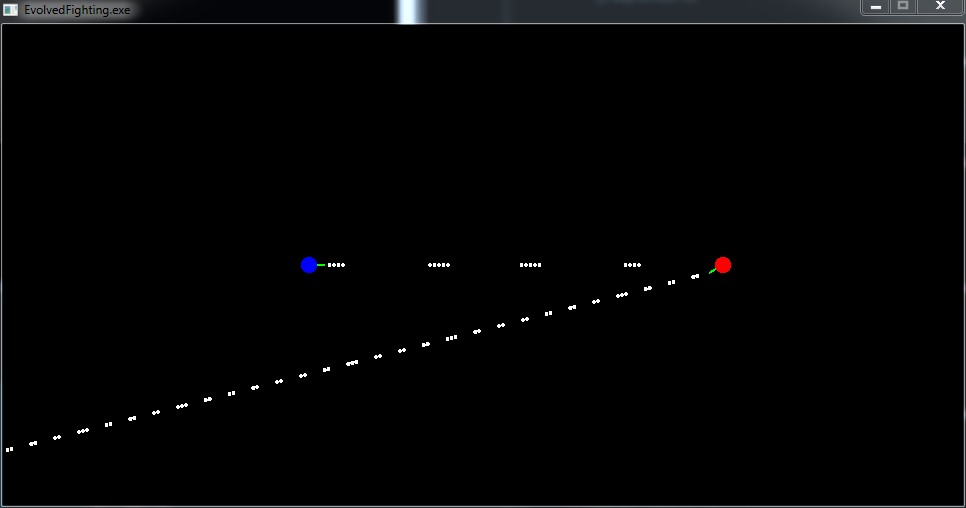
\includegraphics[width=0.5\textwidth]{MaxMax(L)vMinMax(R)g-25}
\end{figure}

\begin{figure}[H]
\centering
\caption{MaxMax(L) vs. MinMin(R): Generation 95}
\label{fig:pic2}
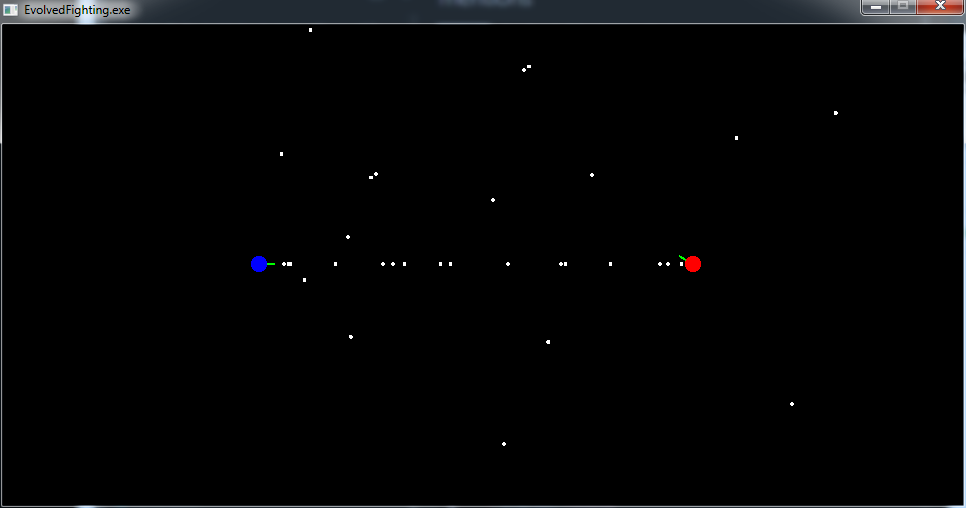
\includegraphics[width=0.5\textwidth]{MaxMax(L)vMinMin(R)g-95}
\end{figure}

%\balancecolumns
% That's all folks!
\end{document}
